\Needspace{8\baselineskip}\originalchapter{2007 期中: 反剪切平衡与自举电流}
题源: Spring 2007 Midterm与Midterm Help, 均为实际公开文件. 整体是一道分分析与编程两部分的综合题. 本章给完整条件、允许的解题分支和真实运行结果; AI辅助的独立实现不是官方答案. ITER参数按2007题模型, 不作当前装置现状.
\begin{exercise}\label{ex:07-mid}
研究ITER用lower hybrid和bootstrap电流稳态运行, 目标fB=.75, 比较所需\ensuremath{\beta}与稳定限.

第一部分A. 不作小\ensuremath{\epsilon}展开, \ensuremath{\Psi}=\ensuremath{\Psi}b\ensuremath{\psi}(x,y),0\ensuremath{\le}\ensuremath{\psi}\ensuremath{\le}1,$R=R_0+ax,Z=ay$, $-1\le x\le1,-\kappa\le y\le\kappa$, $0\le h,f\le1$, p=p0h(\ensuremath{\psi}), $F^2=R_0^2[B_0^2-2\mu_0p+2B_0B_2]$, $B_2=k_0B_0f(\psi)$; 定义 $\beta_0=8\pi^2a^2p_0/(\mu_0I^2)$、$l_0=4\pi\Psi_b/(\mu_0R_0I)$、$C_0=k_0B_0^2a^2R_0^2/(2\Psi_b^2)$, 求无量纲GS.

B. 反坐标\ensuremath{\psi}=\ensuremath{\rho}\ensuremath{{}^{2}}, $x=\sigma_0(1-\rho^2)+\rho\cos(\mu+D\sin\mu)$, $y=[\kappa_0+(\kappa_a-\kappa_0)\rho^2]\rho\sin\mu$, $D=\arcsin\delta_a[\delta_0+(1-\delta_0)\rho^2]\rho^2$. 给\ensuremath{\epsilon}=.32,$\kappa_a=1.7,\delta_a=.4$,\ensuremath{\alpha}=.07, $h=(1-\psi)^2$, $f=(1-\psi)^2(1+3\alpha+2\psi)/(1+3\alpha)$. 给\ensuremath{\epsilon}/\ensuremath{\beta}0求C0,l0,\ensuremath{\sigma}0,\ensuremath{\kappa}0,\ensuremath{\delta}0, 用\ensuremath{\oint}Bpdl=\ensuremath{\mu}0I和四GS矩, 权W=(1,R\ensuremath{-}R0,(R\ensuremath{-}R0)\ensuremath{{}^{2}},Z\ensuremath{{}^{2}}), 矩 $\int_{V_p}W GS\dd V/R^2=0,\ \dd V=R\dd R\dd Z\dd\varphi$.

第二部分A. 编程扫\ensuremath{\beta}0, 画代表磁面. B. $B_0=5.3$ T, $a=2$ m, $R_0=6.2$ m, 求q(\ensuremath{\psi})并找离轴qmin, 选$I$使$q_{\min}=2$; 低于2的空心电流可低\ensuremath{\beta}失稳. H-mode n/n0=(p/p0)$^{1/3}$, 求体平均\ensuremath{\beta}、$q_*=2\pi a^2\kappa_aB_0/(\mu_0R_0I)$、平均自举电流剖面、IB与fB=IB/I, 其中
\begin{equation}
 \beta=\frac{2\mu_0\langle p\rangle_V}{B_0^2},\quad
 J_B=-4.7\frac{R_0^{1/2}q(\rho)T(\rho)}{a^{3/2}B_0\rho^{1/2}}\frac{\dd n}{\dd\rho},\quad
 I_B=\int J_B\dd S,
\end{equation}
磁面平均权dlp/Bp. 扫\ensuremath{\beta}0画fB(\ensuremath{\beta}), 找fB.75. C. 比Troyon \ensuremath{\beta}\ensuremath{\le}.14\ensuremath{\epsilon}\ensuremath{\kappa}a/q*. D. 驱动效率 $I_{CD}\simeq1.2P_{CD}/(n_\parallel^2R_0n_{20})$, 单位MA/MW/m; $n_\parallel=2,n_{20}=1$,40MW够25\%吗, 否则要何fB? E. 同图画平均JB与J\ensuremath{\phi}对\ensuremath{\rho}, 判断重合.

公开补充说明允许改权为 (1,cos\ensuremath{\mu},cos2\ensuremath{\mu},cos3\ensuremath{\mu})或Cartesian几何角权
\begin{equation}
 (W_0,W_1,W_2,W_3)=\left(1,\frac{x}{\sqrt{x^2+y^2}},\frac{x^2-y^2}{x^2+y^2},\frac{x^3-3xy^2}{(x^2+y^2)^{3/2}}\right).
\end{equation}, 并改 $\psi=[36\lambda\rho^2+9(1-\lambda)\rho^4-4\rho^6]/(27\lambda+5)$, \ensuremath{\lambda}可自行选; 也允许退$\psi=\rho^2,q_*=2$的简化, 须说明选择.
\end{exercise}
\begin{solution}
\originalsection{归一化与原件冲突}
原题GS定义另印压力项 $2\mu_0R^2p_\Psi$, 与章\ref{ch:gs}及Lecture12的单系数不一致. 给定F\ensuremath{{}^{2}}恰需单系数才能抵消R0\ensuremath{{}^{2}}压力项, 故明确采用由力平衡导出的标准式, 不是悄悄照双系数算同一模型. 令s=1+\ensuremath{\epsilon}x, 得
\begin{equation}
 L\psi+S=0,\quad L=\partial_x^2+\partial_y^2-\frac\epsilon s\partial_x,\quad
 S=\frac{2\beta_0}{l_0^2}(s^2-1)h_\psi+2C_0f_\psi.
\end{equation}
$h_\psi=-2(1-\psi)$, $f_\psi=-6(1-\psi)(\alpha+\psi)/(1+3\alpha)$. 压力项归一系数来自\ensuremath{\mu}0a\ensuremath{{}^{2}}R0\ensuremath{{}^{2}}p0/\ensuremath{\Psi}b\ensuremath{{}^{2}}=2\ensuremath{\beta}0/l0\ensuremath{{}^{2}}, 所以量纲自洽.

\originalsection{反坐标矩方程}
设 $\mathcal J=x_\rho y_\mu-y_\rho x_\mu$, $G=x_\mu^2+y_\mu^2$, $H=x_\rho x_\mu+y_\rho y_\mu$, \ensuremath{\psi}=g(\ensuremath{\rho}). 无折叠需J>0. 安培约束及积分分部的四矩为
\begin{align}
 &l_0g'(1)\int_0^{2\pi}\frac{G_b}{\mathcal J_bs_b}\dd\mu=4\pi,\\
 &g'(1)\int_0^{2\pi}\frac{W_bG_b}{\mathcal J_bs_b}\dd\mu
 -\int_0^1\!\int_0^{2\pi}\frac{g'(W_\rho G-W_\mu H)}{\mathcal Js}\dd\mu\dd\rho
 +\int_0^1\!\int_0^{2\pi}\frac{WS\mathcal J}{s}\dd\mu\dd\rho=0.
\end{align}
边界$b$取$\rho=1$, 轴心通量因g\ensuremath{{}^{\prime}}趋0无额外边界项. 原权的无量纲等价为1,x,x\ensuremath{{}^{2}},y\ensuremath{{}^{2}}, 其\ensuremath{\rho}/\ensuremath{\mu}导数由x/y直接求; cos谐波则$W_\rho=0,W_\mu=-j\sin(j\mu)$. 这给原指定方法的解析方程, 并允许在同一求解器切换权.

原\ensuremath{\rho}\ensuremath{{}^{2}}与多项式矩从若干Newton/有界初值未求出可信低残差根, 不包装为成功. 本实现采用官方允许cos权与\ensuremath{\lambda}=.2分支, \ensuremath{\epsilon}=2/6.2=.3225806与米制几何一致, .32是题圆整. g\ensuremath{{}^{\prime}}在内部正, 实際求五参数方程并用离轴最小q=2约束选I.

\originalsection{磁面平均、电流和压力}
$F/(B_0R_0)=\sqrt{1-2\mu_0p_0h/B_0^2+2k_0f}$,
\begin{equation}
 q(\rho)=\frac{a^2F}{2\pi R_0\Psi_bg'}\int_0^{2\pi}\frac{\mathcal J}{s}\dd\mu,\quad
 \langle Q\rangle_\rho=\frac{\int Qs\mathcal J\dd\mu}{\int s\mathcal J\dd\mu}.
\end{equation}
这两个权分别J/s与sJ, 不可混用. 平均\ensuremath{\beta}按环体积权sJ, 总I/IB按截面J. 取电子离子同温p=2nT, 题n\ensuremath{\propto}h$^{1/3}$给 $Tdn/\dd\rho=(p_0/6)\dd h/\dd\rho$; 自举电流的n0消去. $J_\varphi=[\mu_0R^2p_\Psi+FF_\Psi]/(\mu_0R)$, 从同一GS求. 本册$\Psi_b>0$、$\psi$向外增加, 而数值性能的$I,I_B,J_B$采用所选电流方向的正强度. 因而图中总电流定义为
\begin{equation}
 \bar J_{\rm tot}=-\langle J_\varphi\rangle=-\frac{\Psi_b}{\mu_0a^2R_0}\frac{\int S\mathcal J\dd\mu}{\int s\mathcal J\dd\mu}.
\end{equation}
比较$J_B$与$\bar J_{\rm tot}$, 不先取$|J_\varphi|$再平均. 权从原三维矩轴对称化为$2\pi\int W GS\dd R\dd Z/R$, 故前述弱矩的$1/s$一致. 官方Help的Cartesian几何角与反坐标角$\mu$在形变/位移后不同, 本次选择后者权组, 不将两者默认互换.

\originalsection{实际数值与性能判断}
72\ensuremath{\times}192径向/角求积扫\ensuremath{\beta}0, 以fB.75求得下表; 144\ensuremath{\times}768独立加密的五矩最大残差 $8.54\times10^{-13}$.
\begin{center}\begin{tabular}{lrrr}\toprule \ensuremath{\beta}0&l0&C0&\ensuremath{\sigma}0\\\midrule
1.4313301&.86382972&1.4074754&.16171814\\\bottomrule\end{tabular}\quad
\begin{tabular}{lrr}\toprule \ensuremath{\kappa}0&\ensuremath{\delta}0&q*\\\midrule1.4918542&1.3248201&1.8386000\\\bottomrule\end{tabular}\end{center}
离轴\ensuremath{\rho}min=.63034963、qmin2, I=15.8079605MA, p0=1.423153MPa, IB=11.8559704MA, \ensuremath{\beta}=.04554225. 面积电流与安培式一致; 48\ensuremath{\times}128至192\ensuremath{\times}1024重新解参数变化小于 $7\times10^{-13}$, fB变化约 $10^{-9}$. 但五矩是有限形状投影, 强形式GS面积加权相对RMS残差约.16978, 不能称完整PDE高精度解.
\begin{center}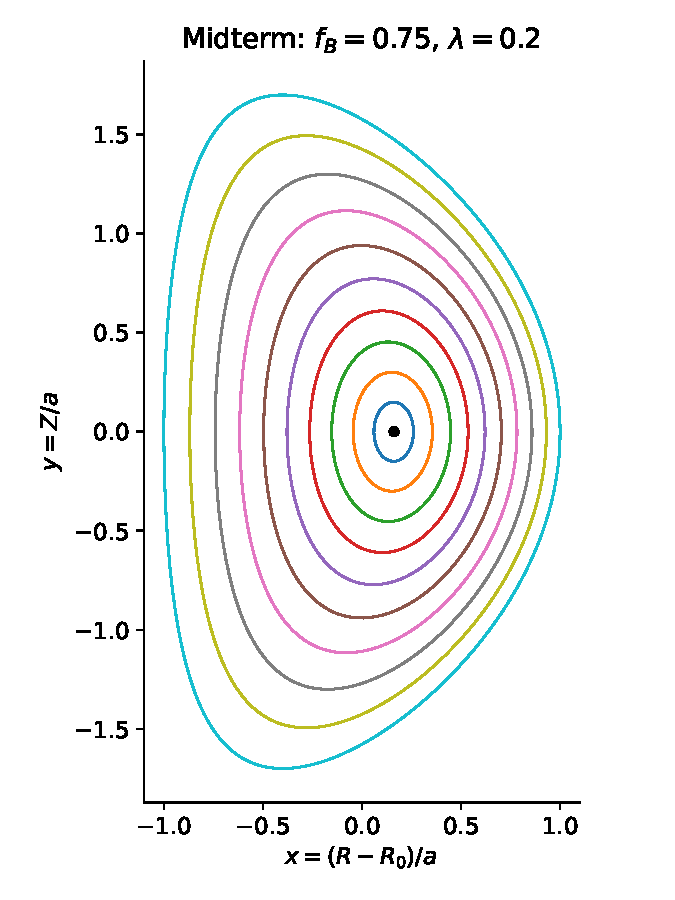
\includegraphics[width=.62\textwidth]{figures/midterm_flux.pdf}\end{center}
以上是实际参数产生的嵌套磁面, 横纵等比例. 实际$f_B(\beta)$如下, Troyon数值比较随后给出.
\begin{center}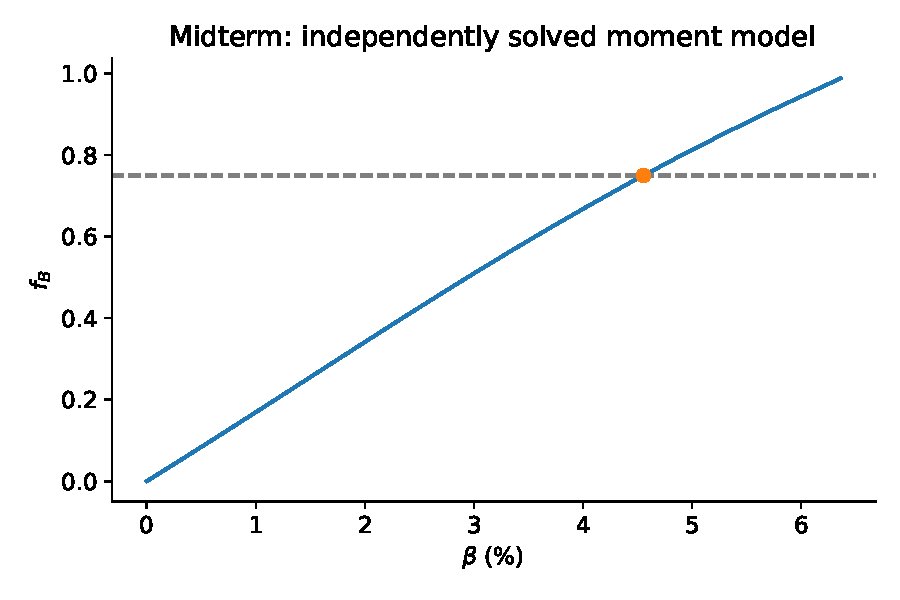
\includegraphics[width=.65\textwidth]{figures/midterm_bootstrap.pdf}\end{center}
Troyon限.04175688<所需.04554225, 此模型的75\%点不满足题给稳定限. 40MW驱动1.93548MA, 余25\%需3.95199MA, 所需PCD=81.67446MW. 若保持这点总I, 要fB至少.8775627; 这不是重新优化平衡后的最低功率.
\begin{center}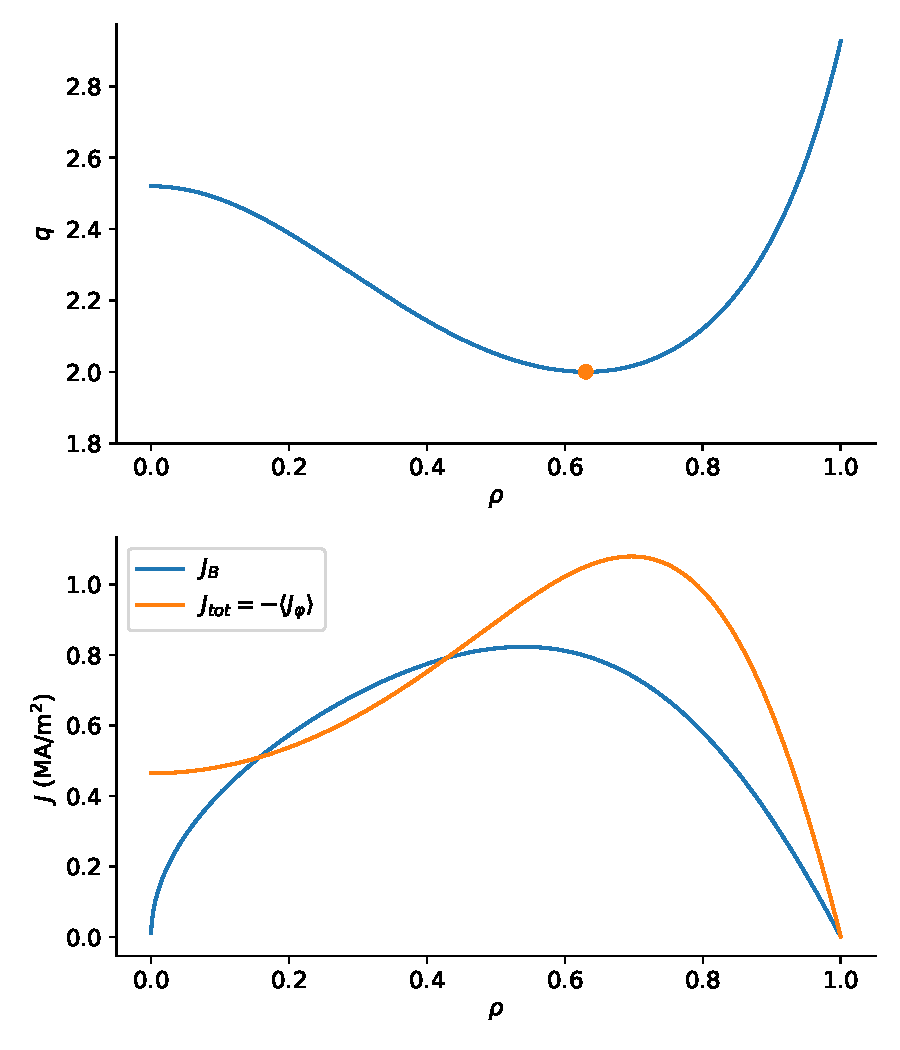
\includegraphics[width=.73\textwidth]{figures/midterm_profiles.pdf}\end{center}
上图q有离轴最低, 下图$J_B$与总$\bar J_{\rm tot}$均空心但峰位和幅度不完全重合, 不能仅因总fB.75就说25\%外驱动在每磁面自动补足. 全部参数扫描、CSV及代码见tools/mhd和qa/numerics; 图来自真实输出, 限制随图保留.
\end{solution}
